% assignment_7.tex - Assignment 7 for Data Fusion class (Fall 2014)
% Chanmann Lim - November 2014

\documentclass[a4paper]{article}

\usepackage[margin=1 in]{geometry}
\usepackage{amsmath}
\usepackage{listings}
\usepackage{graphicx}

\everymath{\displaystyle}

\begin{document}
\title{CS 8790: Report for assignment 7}
\author{Chanmann Lim}
\date{November 10, 2014}
\maketitle

\subsection*{Report:} ~\\
\indent The state of a target moving with constant velocity in 2D coordinate is observed. A sequence of the 2D measurements come with the corresponding \emph{timestamp} at which each observation was taken, the mean $(x, y)$ and the upper triangular elements of the square root of the covariance $sqrtm(R)$ thus observation is now in the form of $(t\_z, z, R)$. \\

One way to start is to initialize our filter with time zero, zero mean and velocity and infinite covariance. \\
\begin{align*}
t = 0, 
x = \begin{bmatrix}
		0 \\ 0 \\ 0 \\ 0
	\end{bmatrix}, 
P = \begin{bmatrix}
		100000000 & 0 & 0 & 0 \\
		0 & 100000000 & 0 & 0 \\
		0 & 0 & 100000000 & 0 \\
		0 & 0 & 0 & 100000000
	\end{bmatrix}
\end{align*} \\
\noindent Yet, combining the estimate and the observation is not feasible unless both measurements are valid at the same \emph{timestamp} which lead us to make prediction of the state of the estimate into the same timestamp as the observation using constant velocity model $F$. \\
\begin{align*}
F \quad (x, P) \to (Fx, FPF')
\end{align*} \\
, where
\begin{align*}
F = \begin{bmatrix}
		1 & 0 & \Delta{}t & 0 \\
		0 & 1 & 0 & \Delta{}t \\
		0 & 0 & 0 & 0 \\
		0 & 0 & 0 & 0
	\end{bmatrix}
\end{align*} \\

\noindent And since the observation comes in lower dimension (without velocity) than the state estimate we have to use transformation matrix $H$ to project down the state estimate before combining them using innovation fusion equation. \\
\begin{align*}
H = \begin{bmatrix}
		1 & 0 & 0 & 0 \\
		0 & 1 & 0 & 0 
	\end{bmatrix}
\end{align*} \\

\paragraph{1.1 } The state of the target at the time of the final observation is : \\
\begin{align*}
\text{mean with standard deviation} = 
	\left(\begin{matrix}
		245.277904 & ,   &    0.002747 \\
    	510.449761 & ,   &    0.001239 \\
      	0.280005 & ,     &  0.000007 \\
      	0.600000 & ,     &  0.000002 \\
	\end{matrix}\right)
\end{align*}
\begin{align*}
x\_final = \begin{bmatrix}
		245.277904 \\
    	510.449761 \\
      	0.280005 \\
      	0.600000 
	\end{bmatrix}
\end{align*}
\begin{align*}
P\_final = \begin{bmatrix}
		0.00000754  &  -0.00000074   &  0.00000002  &  -0.00000000  \\
   		-0.00000074  &   0.00000153  &  -0.00000000  &   0.00000000 \\
    	0.00000002  &  -0.00000000  &   0.00000000  &  -0.00000000 \\
   		-0.00000000  &   0.00000000  &  -0.00000000  &   0.00000000 
	\end{bmatrix}
\end{align*} \\

\paragraph{1.2 } The prediction of the state of the target one hour after the time of the final observation $(t=927.969649836)$ : \\
\begin{align*}
x(4527.969650) = \begin{bmatrix}
		1253.296210 \\
   		2670.451308 \\
      	0.280005 \\
      	0.600000  
	\end{bmatrix}
\end{align*}
\begin{align*}
P(4527.969650) =  \begin{bmatrix}
		    0.00082509  &  -0.00013653  &   0.00000021  &  -0.00000003 \\
   			-0.00013653  &   0.00008861  &  -0.00000004  &   0.00000002 \\
    		0.00000021  &  -0.00000004   &  0.00000000  &  -0.00000000 \\
   			-0.00000003  &   0.00000002  &  -0.00000000   &  0.00000000
	\end{bmatrix}
\end{align*} \\

\paragraph{1.3 } The plots of the sequence of normalized x and y innovations separately : \\
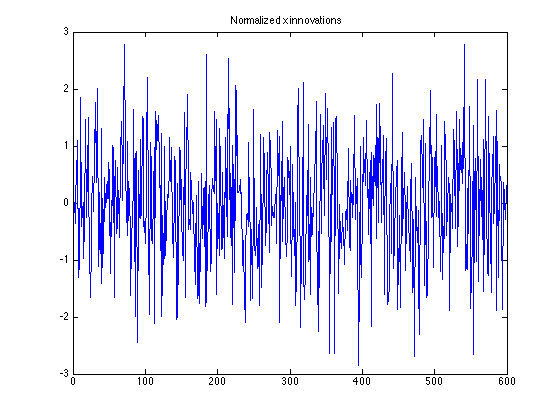
\includegraphics[scale=.4]{target_1_x_inno.png}
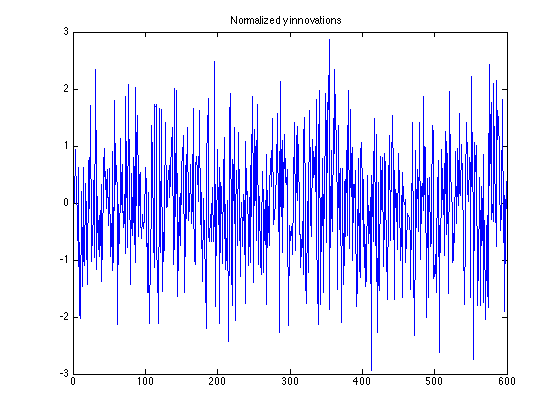
\includegraphics[scale=.4]{target_1_y_inno.png} \\

The normalized x innovations is obtained by $(z - Hx)(1)/\sqrt{S(1,1)}$ and y innovations = $(z - Hx)(2)/\sqrt{S(2,2)}$, where $S$ is the innovation covariance.\\

\paragraph{1.4 } The Percentage of x and y innovations that are less than 0 is $[ 48.50\%, 49.00\% ]$ \\

The plot of the running percentage of the x and y innovations that are less than zero : \\
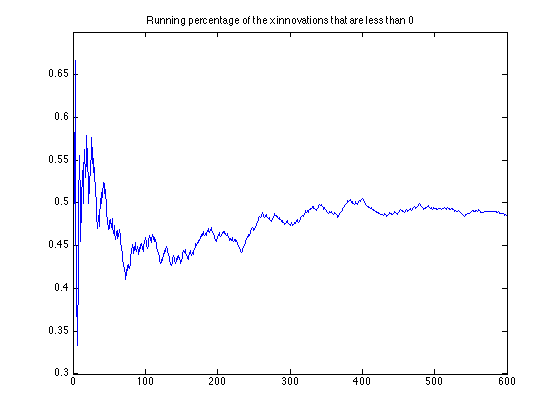
\includegraphics[scale=.4]{target_1_x_running.png}
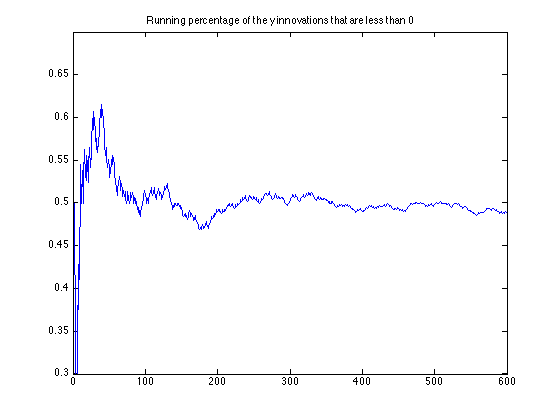
\includegraphics[scale=.4]{target_1_y_running.png} \\

For the second dataset, \texttt{Target2.txt}, the motion of the target deviates slightly from true constant velocity and the uncertainty increases thus in order to account for the deviation we will have to make the covariance bigger by incorporating the process noise covariance matrix $Q$ while predicting the state estimate into the future using the previous kinematic model.

\newpage
\subsection*{Appendix:}
\lstinputlisting[language=Matlab, title=\lstname, basicstyle=\footnotesize]{assignment_7.m}
\lstinputlisting[language=Matlab, title=\lstname, basicstyle=\footnotesize]{filter_7.m}
\lstinputlisting[language=Matlab, title=\lstname, basicstyle=\footnotesize]{get_observation.m}
\lstinputlisting[language=Matlab, title=\lstname, basicstyle=\footnotesize]{predict.m}
\lstinputlisting[language=Matlab, title=\lstname, basicstyle=\footnotesize]{update.m}
\lstinputlisting[language=Matlab, title=\lstname, basicstyle=\footnotesize]{report.m}

\end{document}